\begin{frame}{}
    \LARGE Generative AI for Science: \textbf{Drug Discovery}
\end{frame}

\begin{frame}[allowframebreaks]{Drug Discovery}
    \begin{figure}
        \centering
        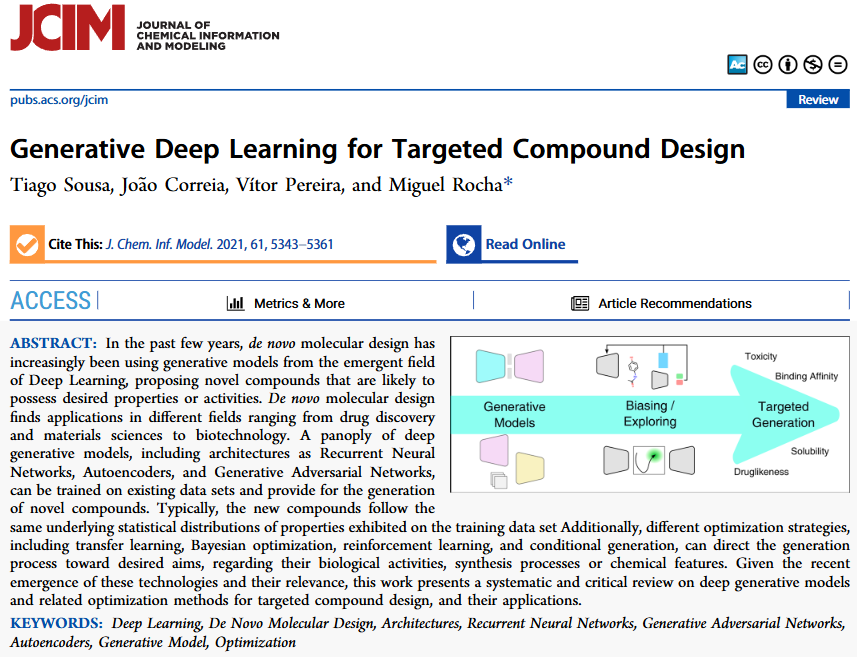
\includegraphics[height=0.8\textheight,width=1\textwidth,keepaspectratio]{images/science/drug-discovery-paper.png}
    \end{figure}
    [Source: \href{https://pubs.acs.org/doi/epdf/10.1021/acs.jcim.0c01496?ref=article_openPDF}{JCIM}]

    \framebreak

    \textbf{Where We Are}
    \begin{itemize}
        \item Drug discovery is the process of finding new medicines.
        \item It involves identifying potential drug candidates, testing them, and bringing them to market.
        \item Traditional methods are slow and expensive, often taking over a decade and billions of dollars.
    \end{itemize}

    \framebreak

    \textbf{Where We Are Going}
    \begin{itemize}
        \item Generative AI can speed up drug discovery by predicting how molecules will behave and interact.
        \item AI can analyze large datasets to find patterns and suggest new drug candidates.
        \item This could lead to faster development of new treatments for diseases.
    \end{itemize}

    \framebreak
    
    \begin{itemize}
        \item Understand how generative AI integrates into the drug discovery pipeline (e.g., SMILES $\rightarrow$ molecules $\rightarrow$ optimization).
        \item Recognize real-world successes of generative AI in drug discovery.
        \item Identify current challenges and hurdles in applying generative AI to this field.
    \end{itemize}

    \framebreak

    \begin{figure}
        \centering
        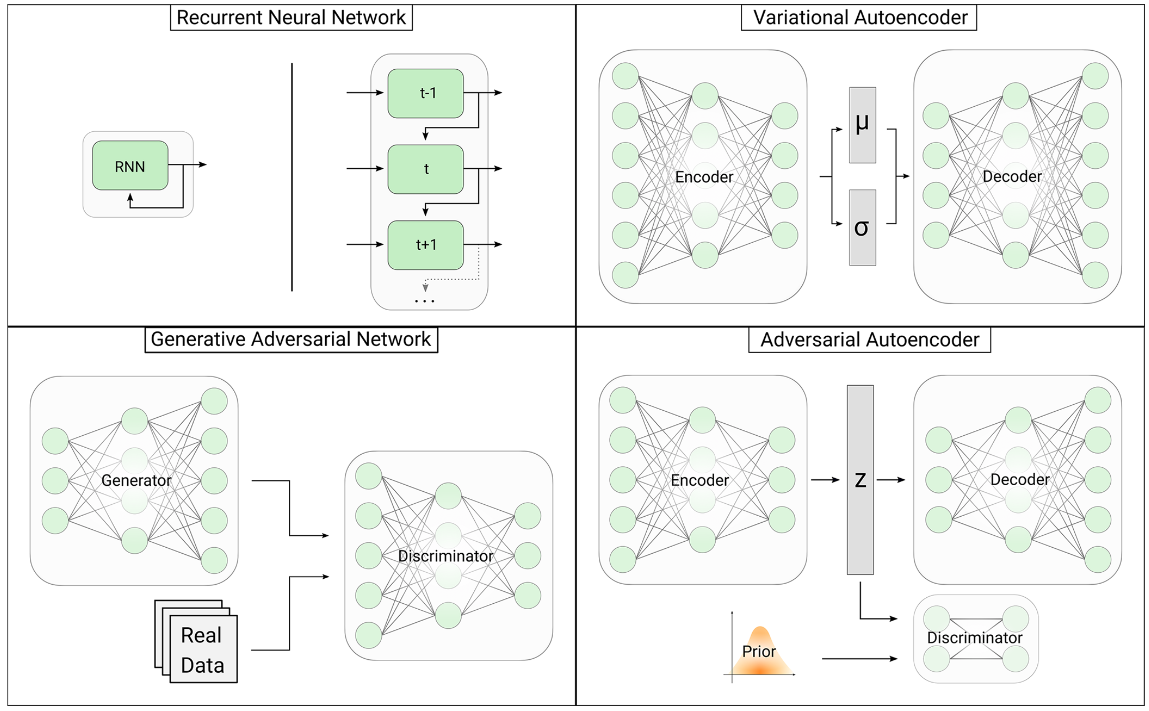
\includegraphics[height=0.9\textheight,width=1\textwidth,keepaspectratio]{images/science/drug-discovery-architecture.png}
    \end{figure}

    \framebreak

    \begin{figure}
        \centering
        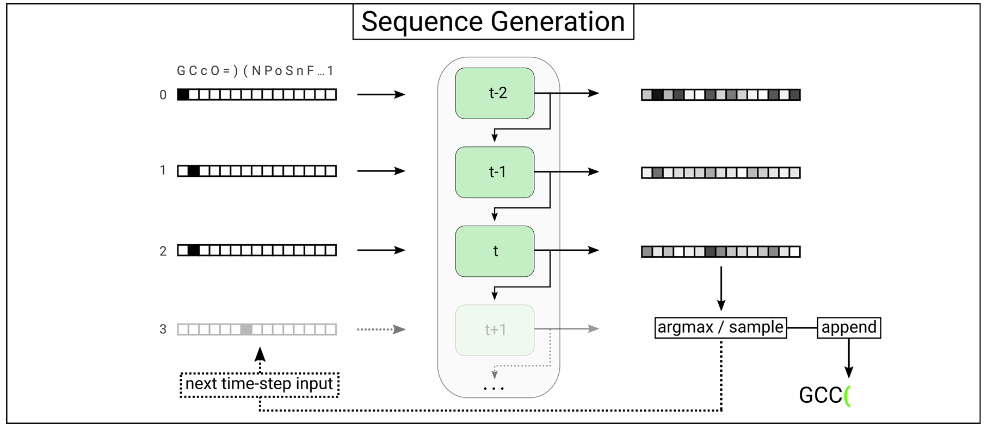
\includegraphics[height=0.8\textheight,width=1\textwidth,keepaspectratio]{images/science/drug-discovery-sequence-gen.png}
        \caption*{Three layer RNN, unfolded over four time-steps.}
    \end{figure}

    \framebreak
    
    \begin{figure}
        \centering
        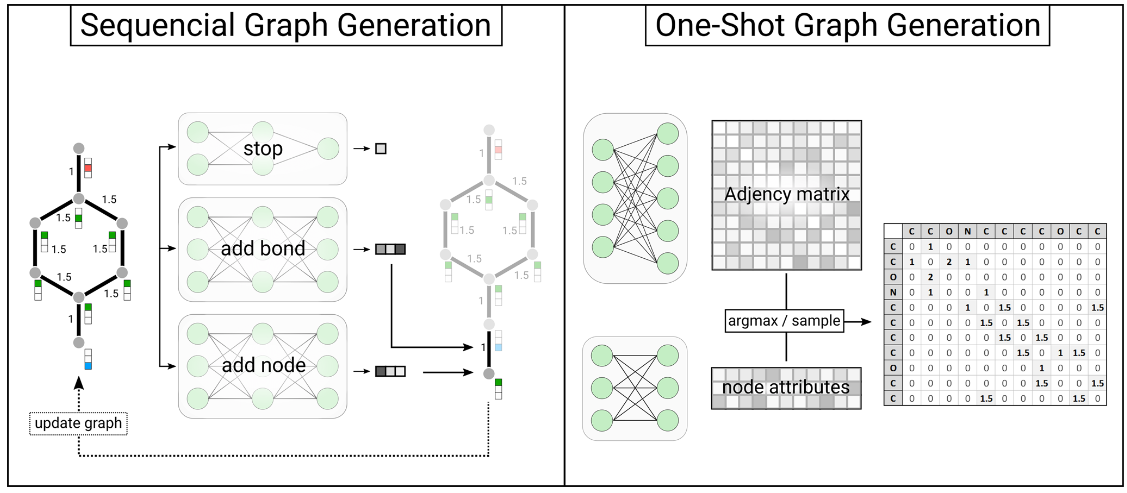
\includegraphics[height=0.65\textheight,width=1\textwidth,keepaspectratio]{images/science/drug-discovery-seq-graph.png}
        \caption*{Left: In sequential graph generation, a graph is built by evaluating a current partial graph, adding a node/edge and repeating until the networkoutputs a stop signal. Right: In the one-shot generation of graphs, probabilities over the full adjacency matrix and node/edge attribute tensors areproduced.}
    \end{figure}

    \framebreak
    
    \begin{figure}
        \centering
        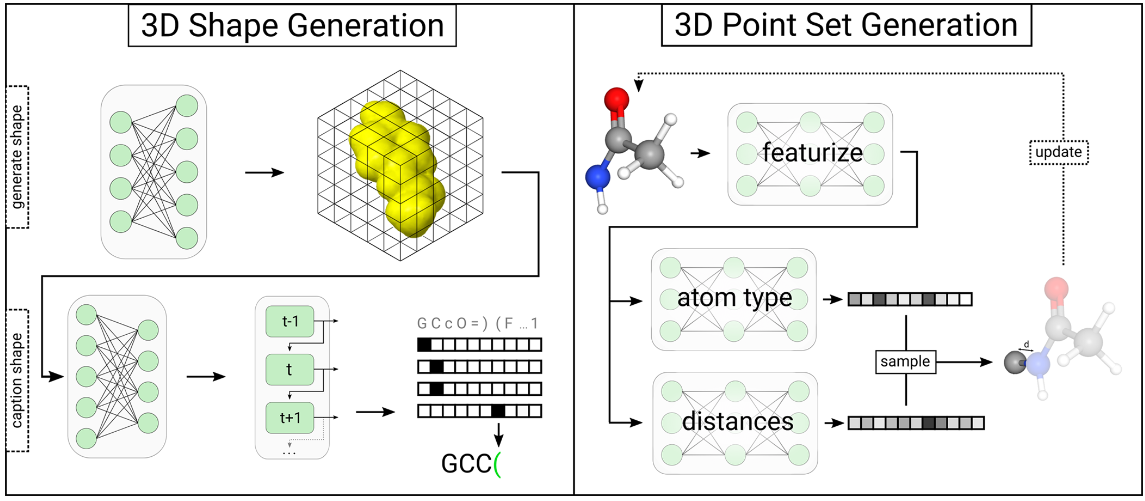
\includegraphics[height=0.65\textheight,width=1\textwidth,keepaspectratio]{images/science/drug-discovery-3d-shape-gen.png}
        \caption*{Left: General procedure for the generation of 3D shapes as proposed by Skalic et al. Right: General process for generating molecules as 3D point sets,proposed by Gebauer et al.}
    \end{figure}

    \framebreak
    
    \begin{figure}
        \centering
        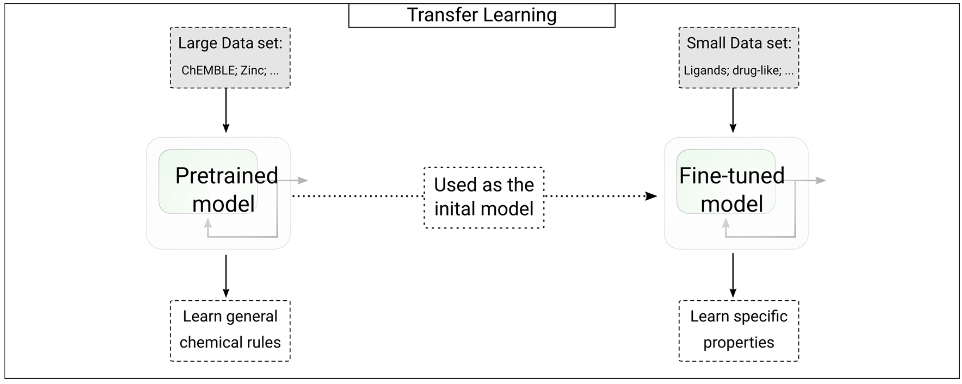
\includegraphics[height=0.65\textheight,width=1\textwidth,keepaspectratio]{images/science/drug-discovery-transfer-learning.png}
        \caption*{In transfer learning, a general model is first trained on a large data set and then fine-tuned toward generating the desired properties with asmaller, focused, data set.}
    \end{figure}

    \framebreak
    
    \begin{figure}
        \centering
        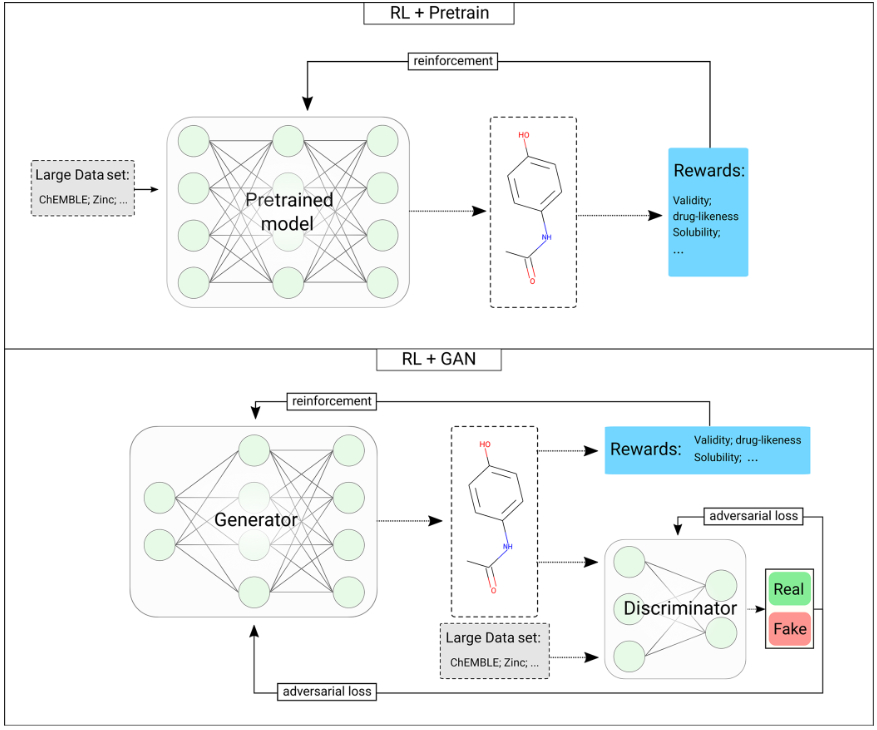
\includegraphics[height=0.74\textheight,width=1\textwidth,keepaspectratio]{images/science/drug-discovery-rl-pretrain-gan.png}
        {\footnotesize
        \caption*{Top: Pretraining with maximum likelihood, then optimizing with RL for specific properties. Bottom: RL and GANs enable directed molecule generation toward desired objectives.}
        }
    \end{figure}

    \framebreak
    
    \begin{figure}
        \centering
        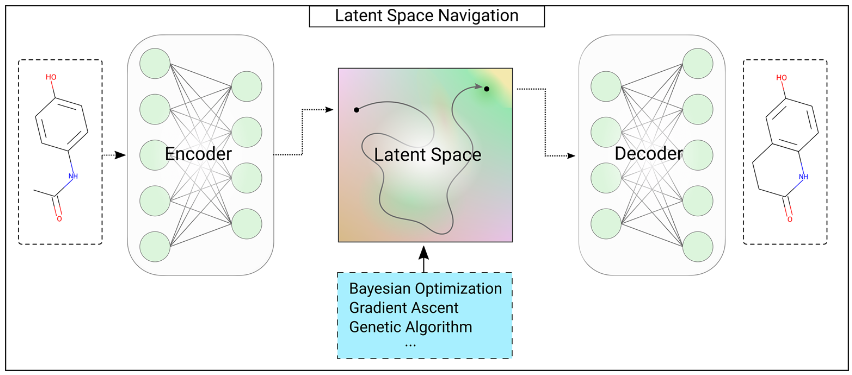
\includegraphics[height=0.75\textheight,width=1\textwidth,keepaspectratio]{images/science/drug-discovery-latent-space.png}
        \caption*{Here, the latent space of an AE is used as a reversible and continuous molecular representation allowing for the application of variousoptimization algorithms.}
    \end{figure}

    \framebreak
    
    \begin{figure}
        \centering
        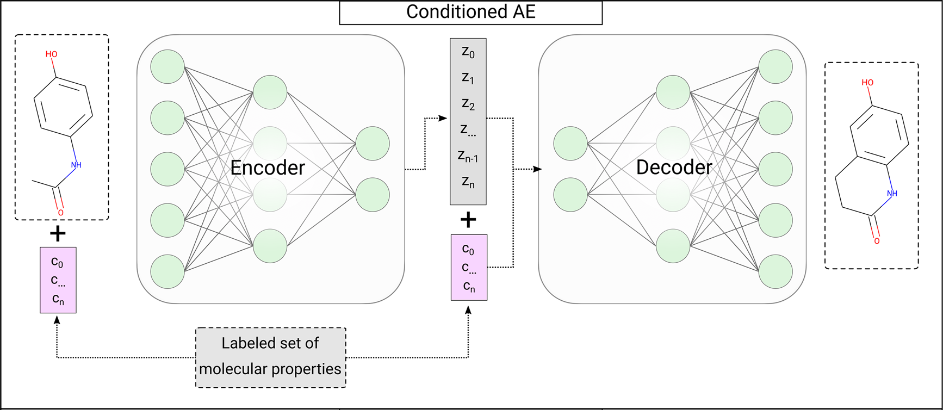
\includegraphics[height=0.75\textheight,width=1\textwidth,keepaspectratio]{images/science/drug-discovery-conditioned-ae.png}
        \caption*{In conditioned generation, desired properties are provided as inputs during training, enabling the model to generate molecules with targeted properties.}  
    \end{figure}

    \framebreak
    
    \begin{figure}
        \centering
        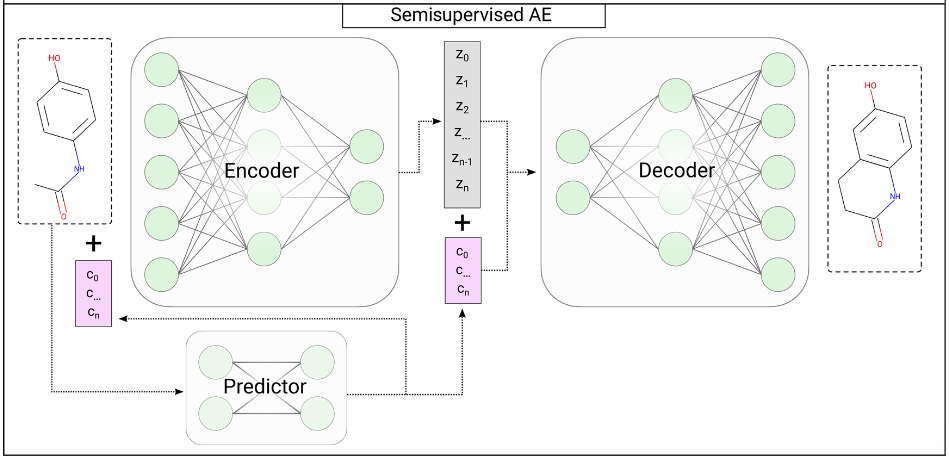
\includegraphics[height=0.75\textheight,width=1\textwidth,keepaspectratio]{images/science/drug-discovery-semisup-ae.png}
        \caption*{In semisupervised conditioned generation, a predictor network infers missing properties for unlabeled data.}
    \end{figure}

    \framebreak

    \begin{center}
        \href{https://www.youtube.com/watch?v=4CHuIyW1oNg}{\texttt{Generative AI for Molecular Design and Synthesis}}
    \end{center}

    \framebreak
    \textbf{Limitations}
    \begin{itemize}
        \item \textbf{Synthetic feasibility}: Not all AI-generated molecules can be easily synthesized in the lab.
        \item \textbf{Lab validation}: Experimental validation is required to confirm predicted properties and efficacy.
        \item \textbf{Regulatory barriers}: Approval processes for new drugs are lengthy and complex.
        \item \textbf{Data bias}: Training data may not represent all relevant chemical space, leading to biased predictions.
        \item \textbf{Model collapse}: Generative models can produce limited diversity or converge to trivial solutions.
    \end{itemize}
\end{frame}